\chapter{ Констукторский раздел}
\label{cha:design}
 Рассмотрим задачу смешения цветов в контексте наложения двух и более изображений.
 
  \section{Идея}
 Данная задача особенна тем, что над всеми пикселями выполняются одинаковые операции. Исходя из этого, можно разбить исходное изображение на канальные изображения, а их, в свою очередь, на блоки пикселей, над которыми можно производить одну операцию в один момент времени. Таким образом, приходим к необходимости использования векторных инструкций для ускорения обработки изображений.

 \section{Алгоритм }
 При построении алгоритма следует учесть, что 
 \begin{enumerate}
 	\item все вычисления выполняются векторными инструкциями блоками..
 	\item изображение помимо RGB-параметров может иметь также маску и транспарентность. Под маской будем понимать канал, представляющий собой информацию о том, какие области изображения необходимо смешать, под транспарентностью - общую прозрачность изображения.
\end{enumerate}

\begin{figure}[ht!]
	\centering{ 
		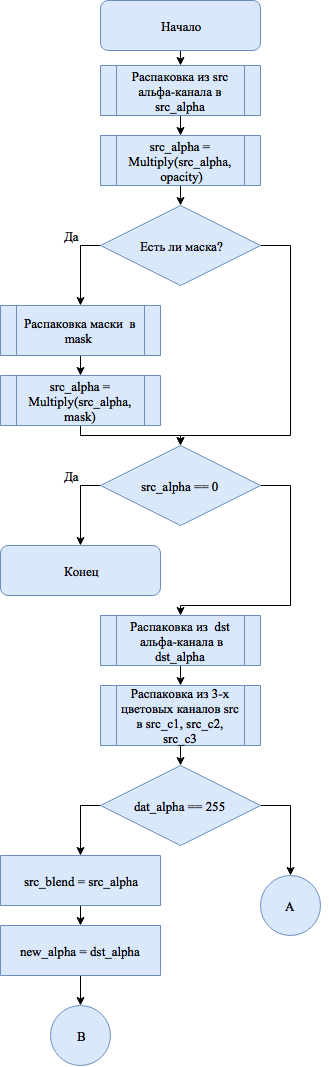
\includegraphics[width=0.49\textwidth]{img/alg.png}
		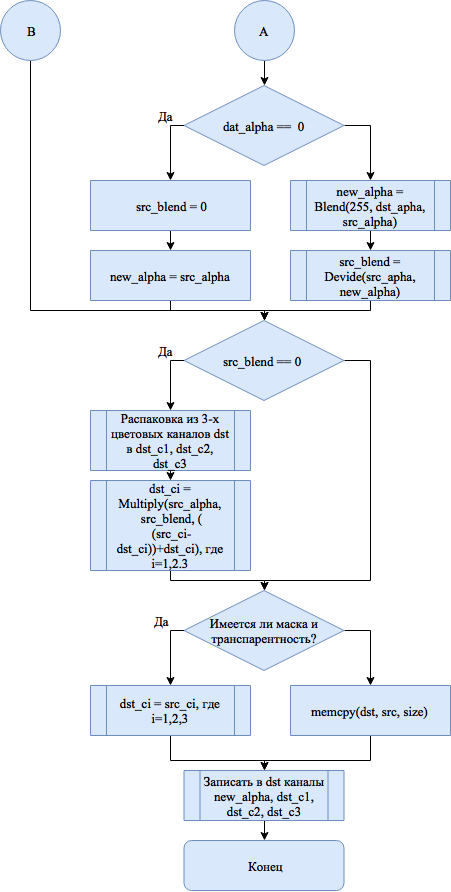
\includegraphics[width=0.49\textwidth]{img/alg-2.png}
		\caption{Схема алгоритма.}}
\end{figure}

Алгоритм представлен на рисунке 2.1 ниже.
